\subsection{Internet of Things (IoT)}
\label{subsec:03_IoT}

Figure \ref{fig:iot_market} shows the predicted market impact of IoT in billion U.S. dollars in each category.
Not only is IoT relevant for the Industry 4.0 with smart factories or the move toward smart cities. IoT also
impacts everyday life with smart homes, vehicles and healthcare. This section aims to present collected solutions on how  blockchain technology can help with security with regards to IoT and its applications.


\begin{figure}[ht!]
  \begin{center}
    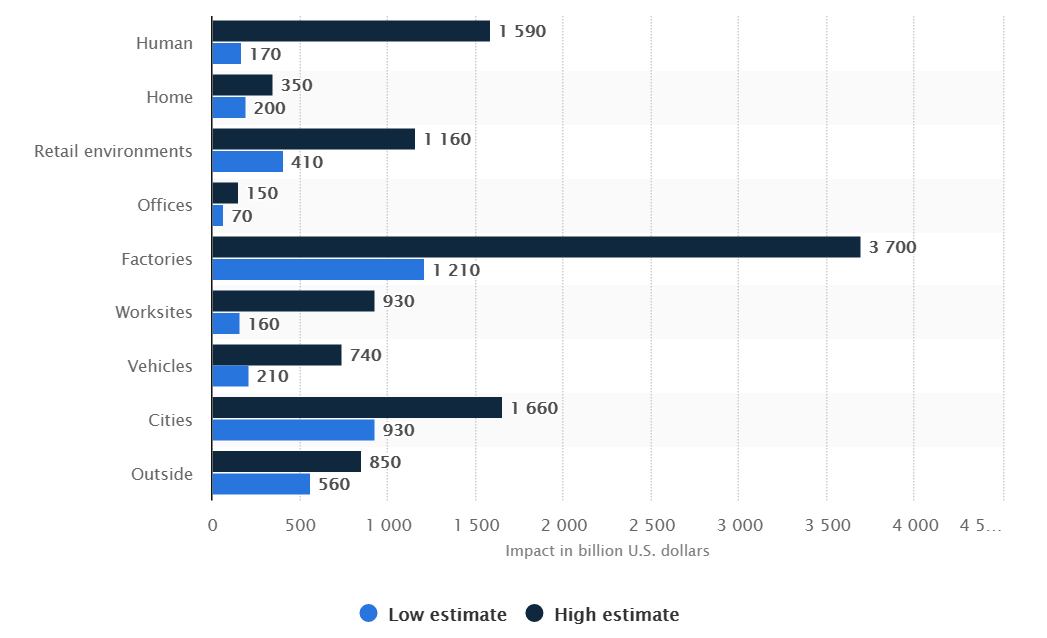
\includegraphics[scale=0.6]{Talk7/img/iot/iot_statista}
  \end{center}
  \caption{Iot market impact, Source: \protect\url{https://www.statista.com/statistics/580778/worldwide-internet-of-things-economic-impact-forecast/}~\cite{StatistaIoT} }
  \label{fig:iot_market}
\end{figure}

Banerjee et. al. in \cite{Banerjee2018} state that given the potentially sensitive nature of IoT datasets,
there is a need to develop a standard for sharing IoT datasets among the research and practitioner communities
and other relevant stakeholders. They propose two examples to use blockchain for IoT security. One for IoT dataset sharing using blockchain and another one for
blockchain based firmware detection and self healing of devices.

First, to ensure integrity of the IoT datasets, they propose a Reference Integritiy Metric (RIM) maintained by a blockchain. Whenever a dataset is downloaded, its integrity can be checked using the RIM.
A central hub maintains the references to the repositories of the datasets. Information of the members is also stored in a blockchain.
Lifetime of the shared datasets is in the hand of the repository owner.
As only the RIM is stored in the blockchain and not the datasets themselves, members can still choose to stop sharing their datasets by removing the repositories.
To preserve privacy, they emphasize the use of an automated tool that anonymizes the datasets before they are published.


Second, to ensure firmware integrity, they also propose a system with RIM checking and blockchain.
Firmware is considered the root of trust. Starting with the bootloader, it checks wether the next software (e.g., the operating system) can be loaded.
But firmware must allow for updates, which opens up a window to compromise the RIM of the firmware. By using blockchain, the firmware history can be tracked and compromised devices can be detected and forced to rollback their
version to the last valid entry.

Khan et. al. in \cite{Khan2018} review and classify security issues for IoT. They discuss various blockchain solutions for IOT:

\begin{itemize}
  \item {\textbf{Address Space}: With blockchain more addresses can be used than with IPv6. Blockchain has a 160-bit address space, while IPv6 offers a 120-bit address space.
  Also, many IoT devices are constrained in memory and computation capacity, and therefore will be unfit to run an IPv6 stack.}
  \item {\textbf{Identity of Things (IDoT) and Governance}: IoT devices often change ownership along the supply chain or when resold. Also IoT devices have many relationships. Those relationships can be \textit{device-to-human}, \textit{device-to-device} or \textit{device-to-service}. Further relationships could be \textit{deployed by}, \textit{shipped by}, \textit{used by}. With blockchain, such challenges can be solved efficiently and securely.}
  \item {\textbf{Data authentication and Integrity}: Data transmission of IoT devices connected to a blockchain will always be  cryptographically proofed and signed by the true sender.}
  \item {\textbf{Authentication, Authorization, and Privacy}: Smart contracts offer the ability for more effective authentication and authorization rules than traditional methods like OAuth 2.0. Data privacy can be enforced by programming access rules into smart contracts. These rules then determine who has the right to update, patch or reset the IoT devices. Also, service and repair requests and change of ownership can be initiated that way. }
  \item {\textbf{Secure Communications}: IoT communication protocols like HTTP and MQTT are not secure by design. They have to be wrapped by security protocols to make them secure, like with TLS for HTTPS.
  With blockchain the complexity of PKI and its management is simplified. Every IoT device connected to the blockchain will have its own unique GUID and asymmetric key pair. }
\end{itemize}


Dorri et. al. in \cite{Dorri2017SmartHome} present a use case for blockchain in a smart home. In their use case, each smart home is equipped with an always online, high resource device, called the ``miner''. It is responsible for handling all communication within and external to the home.
The miner mines a private and secure blockchain used for controlling and auditing communications. To address challenges of power consumption for the Proof-of-Work (POW), they propose a framework based on trust to limit energy consumption to make their solution more suitable in the context of IoT.

The design consists of three core components: the smart homes, a cloud storage, and an overlay.
Smart homes build and overlay with the Service Provider (SP). Smart homes are clustered and, in each cluster, one home is selected as Cluster Head (CH).
They maintain a public blockchain and two key lists. One list contains the private keys of overlay users that are allowed to access data for the smart homes connected to this cluster.
The other list holds the public keys of smart homes that are allowed to be accessed.
Finally, the cloud storage stores and shares data of the smart home devices.

The local blockchain in the smart homes keeps track of transactions and has a policy header to enforce users' policy for incoming and outgoing transactions.
The policy header consist of four parameters. The first is the requesters public key, the second is the requested action (e.g., to store or access data in the cloud storage), the third is the ID of the device inside the smart home,
and the last parameter is to indicate the action that should be done for the transaction that matches with the previous properties (e.g., deny or allow the transaction).
The miner in each smart homes authenticates, authorizes, and audits transactions.
